\section{\textbf{Dependencies in Dyadic Data}}

Relational, or dyadic, data provide measurements of how sets of actors relate to one another. Typically, pairs of actors are examined. These pairs are called \textit{dyads}. Such data can be arranged as a directed dyadic design in which the unit of analysis is some set of $n$ actors that have been paired together to form a matrix of dyads, i. e., represented as a $n \times n$ matrix, $\mathbf{Y}$, with diagonals typically undefined. The $ij^{th}$ entry defines the relationship of $i$ and $j$ and can be continuous or discrete. It can also be symmetric (known as undirected) or asymmetric (called directed). This is not the stacked dyad structure normally found in social science, but it is equivalent and presents a format in which the interdependencies are exposed and transparent. The standard statistical approach to these data uses a linear or generalized linear model (GLM) which assumes that each of the dyadic observations is conditionally independent on observed regressors, even though events and relationships between these actors is most often \textit{inter}dependent. 

\begin{figure}
	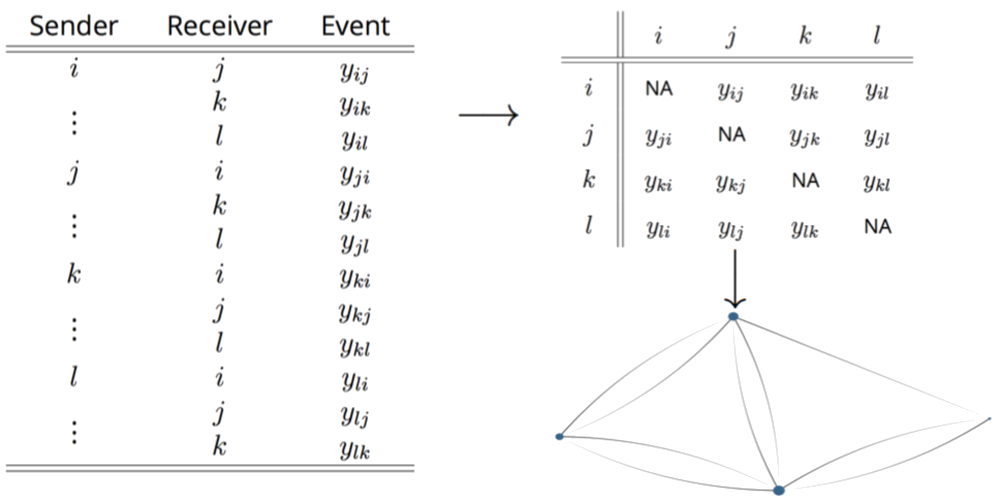
\includegraphics[width=1\textwidth]{df_adj_net3.png}
	\caption{Relational data from dyadic designs to networks}
	\label{fig:ddToNet}
\end{figure}

One important dependency is nodal dependency, whereby each actor has similar interactions with many of its partners, leading to significant heterogeneity in activity levels across nodes. An important implication of this across-node heterogeneity is within-node homogeneity of ties: the values across a row, say $\{y_{ij},y_{ik},y_{il}\}$, are similar to each other because each has a common sender. If a sender $i$ is more active active in the network than other senders, it will have greater homogeneity of its linkages. More popular targets show greater similarity across linkages in a given column, $\{y_{ji},y_{ki},y_{li}\}$. Actors which are more likely to send ties in a network are also more likely to receive them. As a result the rows and columns in an adjacency matrix may be correlated. Another structural interdependence is reciprocity. This is a second-order, or dyadic dependency whereby values of $y_{ij}$ and $y_{ji}$ are correlated. If the data are simply stacked dyads in some arbitrary order, this kind of dependency is harder to visualize, but exists nonetheless.

The presence of these interdependencies in relational data complicates the practical assumption of observational independence.  Inferences drawn from models that ignore potential interdependencies between dyadic observations face a number of well-known challenges: a) biased estimates of the effect of independent variables, b) uncalibrated confidence intervals, and c) poor predictive performance. By ignoring these potential interdependencies, we often ignore important features of the problem under study. The study of international relations is founded on the relations among actors. Why ignore the interdependencies that led to the study of IR in the first place?

The additive part described above does not handle third-order dependency. A third-order dependency is the dependency between triads, not dyads. Third-order effects can arise from the presence of some set of shared attributes between actors that affects their probability of interacting with one another. Individuals try to close triads because this is thought to be a more stable or preferable social situation \citep{wasserman:faust:1994,zinnes:1967}.

For example, a common finding is that democracies are more likely to form trade agreements with one another. Both geographic proximity and a country's political system are examples of homophily, which captures the idea that the relationships between actors with similar characteristics in a network are likely to be stronger than nodes with different characteristics. Homophily can be used to explain the emergence of patterns such as transitivity (``a friend of a friend is a friend'') and balance (``an enemy of a friend is an enemy''), which have a long history in international relations. A binary network where actors tend to form ties based on shared characteristics  often leads to a network with a high number of ``transitive triads'' in which  sets of actors $\{i,j,k\}$ are each linked to one another. Thus, unless we specify a list of exogenous variables that determine this prevalence of triads, the probability of $j$ and $k$ forming a tie is not independent of the ties that already exist between those actors and others.

Another third-order dependence pattern is stochastic equivalence. Actors $i,j$ are stochastically equivalent if the probability of $i$ relating to every other actor is similar to the probability for $j$. Equivalence implies the existence of groups of nodes in a network with similar relational patterns.  Recent work has found stochastic equivalence to be important \citep{manger:etal:2012}. Latent variables can account for third-order dependence patterns within the context of the SRRM. These models assume that relationships between nodes are mediated by a small number ($K$) of node-specific unobserved latent variables. 

\section{\textbf{Additive and Multiplicative Effect Models for Networks}}

The AME approach can be used to conduct inference on cross-sectional and longitudinal networks with binary, ordinal, or continuous linkages. It is flexible and easy to use for analyzing the kind of relational data often found in social science.  It accounts for nodal and dyadic dependence patterns, as well as higher-order dependencies such as homophily and stochastic equivalence.  We do not know whether interdependence dominates international relations, but as noted by Thoreau in reference to rumors that dairymen on strike were watering down milk: ``\ldots some circumstantial evidence is very strong, as when you find a trout in the milk.''  At a very minimum, it is necessary to examine whether there is interdependence since it challenges substantive arguments as well as statistical modeling \citep{snijders:2011}. Ignoring the assumption of independence is a widely-noted shortcoming of many studies, but it continues to be the standard practice in much scholarship. Fortunately, it is easy to empirically examine dependencies in relational data.

The additive and multiplicative effects model (AME) can help to eliminate this color-blindness to interdependence. It was introduced in \cite{hoff:2008}; the open-source computer package associated with this approach is \cite{amenpkg}. We describe it below.

Parameter interpretation is straightforward because it has a simple regression basis as shown in Equation~\ref{eqn:ame} which portrays directed matrix \:

\begin{align}
\begin{aligned}
	y_{ij} &= g(\theta_{ij}) \\
	&\theta_{ij} = \bm\beta^{\top} \mathbf{X}_{ij} + e_{ij} \\
	&e_{ij} = a_{i} + b_{j}  + \epsilon_{ij} + \alpha(\textbf{u}_{i}, \textbf{v}_{j}) \text{  , where } \\
	&\qquad \alpha(\textbf{u}_{i}, \textbf{v}_{j}) = \textbf{u}_{i}^{\top} \textbf{D} \textbf{v}_{j} = \sum_{k \in K} d_{k} u_{ik} v_{jk}. \\
\label{eqn:ame}
\end{aligned}
\end{align}

With this framework, it is straightforward to model dyadic observations as conditionally independent given $\bm\theta$, where $\bm\theta$ depends on the the unobserved random effects modeled to account for the potential \first, \second, and \third-order dependencies. In Equation~\ref{eqn:srmCov}, $a_{i} + b_{j}  + \epsilon_{ij}$ represent the additive random effects in this framework and account for sender, receiver, and within-dyad dependence. The multiplicative effects, $\textbf{u}_{i}^{\top} \textbf{D} \textbf{v}_{j}$, capture higher-order dependence patterns in $\bm\theta$ after accounting for any known covariate information. A Bayesian procedure in which parameters are iteratively updated using a Gibbs sampler is available in the \pkg{amen} $\sf{R}$ package to estimate this type of generalized linear mixed effects model from Gaussian, binary, ordinal, and other relational data types.

\subsection{\textbf{Social Relations Model: Additive Part of AME}}

\citet{warner:etal:1979} developed a social relations model (SRM), using ANOVA decomposition, that focuses on such dependencies. SRM provides the error structure for the additive effects component of the AME framework. SRM decomposes the variance of dyadic observations in terms of a) heterogeneity across row means (often called out-degree), b) column means (or, in-degree), c) correlation between row and column means, and d) correlations within dyads.  \citet{wong:1982,li:loken:2002} provide a random effects representation of the SRM:

\begin{align}
\begin{aligned}
	y_{ij} &= \mu + e_{ij} \\
	e_{ij} &= a_{i} + b_{j} + \epsilon_{ij} \\
	\{ (a_{1}, b_{1}), \ldots, (a_{n}, b_{n}) \} &\simiid N(0,\Sigma_{ab}) \\ 
	\{ (\epsilon_{ij}, \epsilon_{ji}) : \; i \neq j\} &\simiid N(0,\Sigma_{\epsilon}), \text{ where } \\
	\Sigma_{ab} = \begin{pmatrix} \sigma_{a}^{2} & \sigma_{ab} \\ \sigma_{ab} & \sigma_{b}^2   \end{pmatrix} \;\;\;\;\; &\Sigma_{\epsilon} = \sigma_{\epsilon}^{2} \begin{pmatrix} 1 & \rho \\ \rho & 1  \end{pmatrix},
\label{eqn:srmCov}
\end{aligned}
\end{align}

wherein $\mu$ is the density of a network, and $e_{ij}$ represents residual variation in each cell (or dyad). The residual variation has three separate parts: a)   row/sender effects ($a_{i}$), b)  column/receiver effects ($b_{j}$), and c) within-dyad effects ($\epsilon_{ij}$). The row and column effects are modeled jointly to account for correlation in how active an actor is in sending and receiving ties. Heterogeneity in the row and column means is modeled by $\sigma_{a}^{2}$ and $\sigma_{b}^{2}$, respectively.  $\sigma_{ab}$ describes whether actors which send a lot of ties also receive a lot. Second-order dependencies are described by $\sigma_{\epsilon}^{2}$ and a reciprocity, parameter $\rho$. 

The SRM covariance structure described in Equation~\ref{eqn:srmCov} can be incorporated into the systematic component of a GLM framework to produce the social relations regression model (SRRM): $\bm\beta^{\top} \mathbf{X}_{ij} + a_{i} + b_{j} + \epsilon_{ij}$, where $ \bm\beta^{\top} \mathbf{X}_{ij}$ accommodates the inclusion of dyadic, sender, and receiver covariates \citep{hoff:2005}. This is a regression framework with additive, random effects, but it models variances and covariances often seen in relational data. Furthermore, this accommodates a diversity of outcome distributions. In the case of binary data, this can be done by utilizing a random effects logistic (or probit) latent variable representation. 

\subsection{\textbf{Latent Factor Model: Multiplicative Part of AME}}

The latent factor model (LFM) expands the SSRM to include an additional term, $y_{ij}$, $\alpha(u_{i}, u_{j})$, that captures latent third-order characteristics of a network---where $u_{i}$ and $u_{j}$ are node-specific latent variables for symmetric data. General definitions for how $\alpha(u_{i}, u_{j})$ is defined for these latent variable models are shown in Equation~\ref{eqn:latAlpha}. 

\begin{align}
\begin{aligned}
	\alpha(&\textbf{u}_{i}, \textbf{u}_{j}) = \textbf{u}_{i}^{\top} \Lambda \textbf{u}_{j} \\
	&\textbf{u}_{i} \in \mathbb{R}^{K}, \; i \in \{1, \ldots, n \} \text{, where}\\
	 &\Lambda \equiv K \times K \text{ diagonal matrix}
\label{eqn:latAlpha}
\end{aligned}
\end{align}

Many observed  networks exhibit varying degrees of stochastic equivalence and homophily.  In the latent factor model, each actor has an unobserved vector of characteristics, $\textbf{u}_{i} = \{u_{i,1}, \ldots, u_{i,K} \}$, describing each node's behavior in the network. The probability of a tie between $i$ and $j$ depends on the extent to which $\textbf{u}_{i}$ and $\textbf{u}_{j}$ are ``similar'' and on whether the entries of $\Lambda$ are greater or less than zero. Similarity in the latent factors, $\textbf{u}_{i} \approx \textbf{u}_{j}$, corresponds to stochastic equivalence; the eigenvalue determines whether the network exhibits positive or negative homophily. Accordingly, this approach can represent both homophily and stochastic equivalence. 

In directed (asymmetric) networks there are two sets of latent positions, denoted $\textbf{u}$ and $\textbf{v}$, representing the sending and receiving positions separately.  Thus, actors in the network have a vector of latent characteristics describing their behavior as a sender, denoted by $\textbf{u}$, and as a receiver, $\textbf{v}$: $\textbf{u}_{i}, \textbf{v}_{j} \in \mathbb{R}^{K}$. This can alter the probability of an interaction between $ij$ additively: $\textbf{u}_{i}^{\top} \textbf{D} \textbf{v}_{j}$, where $\textbf{D}$ is a $K \times K$ diagonal matrix.

The LFM captures a wide range of interdependence patterns that arise in relational data such as often studied in international relations. 